\lfoot{Autor: Raphael Simsek}
\subsection{Schaltvorschlag}

\subsubsection{Prototyp}
Für den Prototyp wurde zuerst überlegt, wie man am den Schaltvorschlag umsetzen kann. Dafür wurden die Überlegungen aus dem Kapitel 2.1.2 Motorwirkungsgrad herangezogen:
Zitat:
\textit{
Also kurz:
\begin{itemize}
	\item 90\% der max. Drehzahl oder Drehmoment --> hochschalten, wegen niedrigem Wirkungsgrad
	\item niedrige Drehzahl \&\& hohe Last --> hinunterschalten, wegen Verschleiß durch Motorschwingungen
\end{itemize}
}
Diese Skizze beschreibt die Umsetzungsüberlegungen am Beginn der Prototypenphase. Dabei ist auf der horizontalen Achse die Drehzahl und auf der vertikalen Achse das Drehmoment angeschlagen.
\begin{figure}[!htb]\centering
		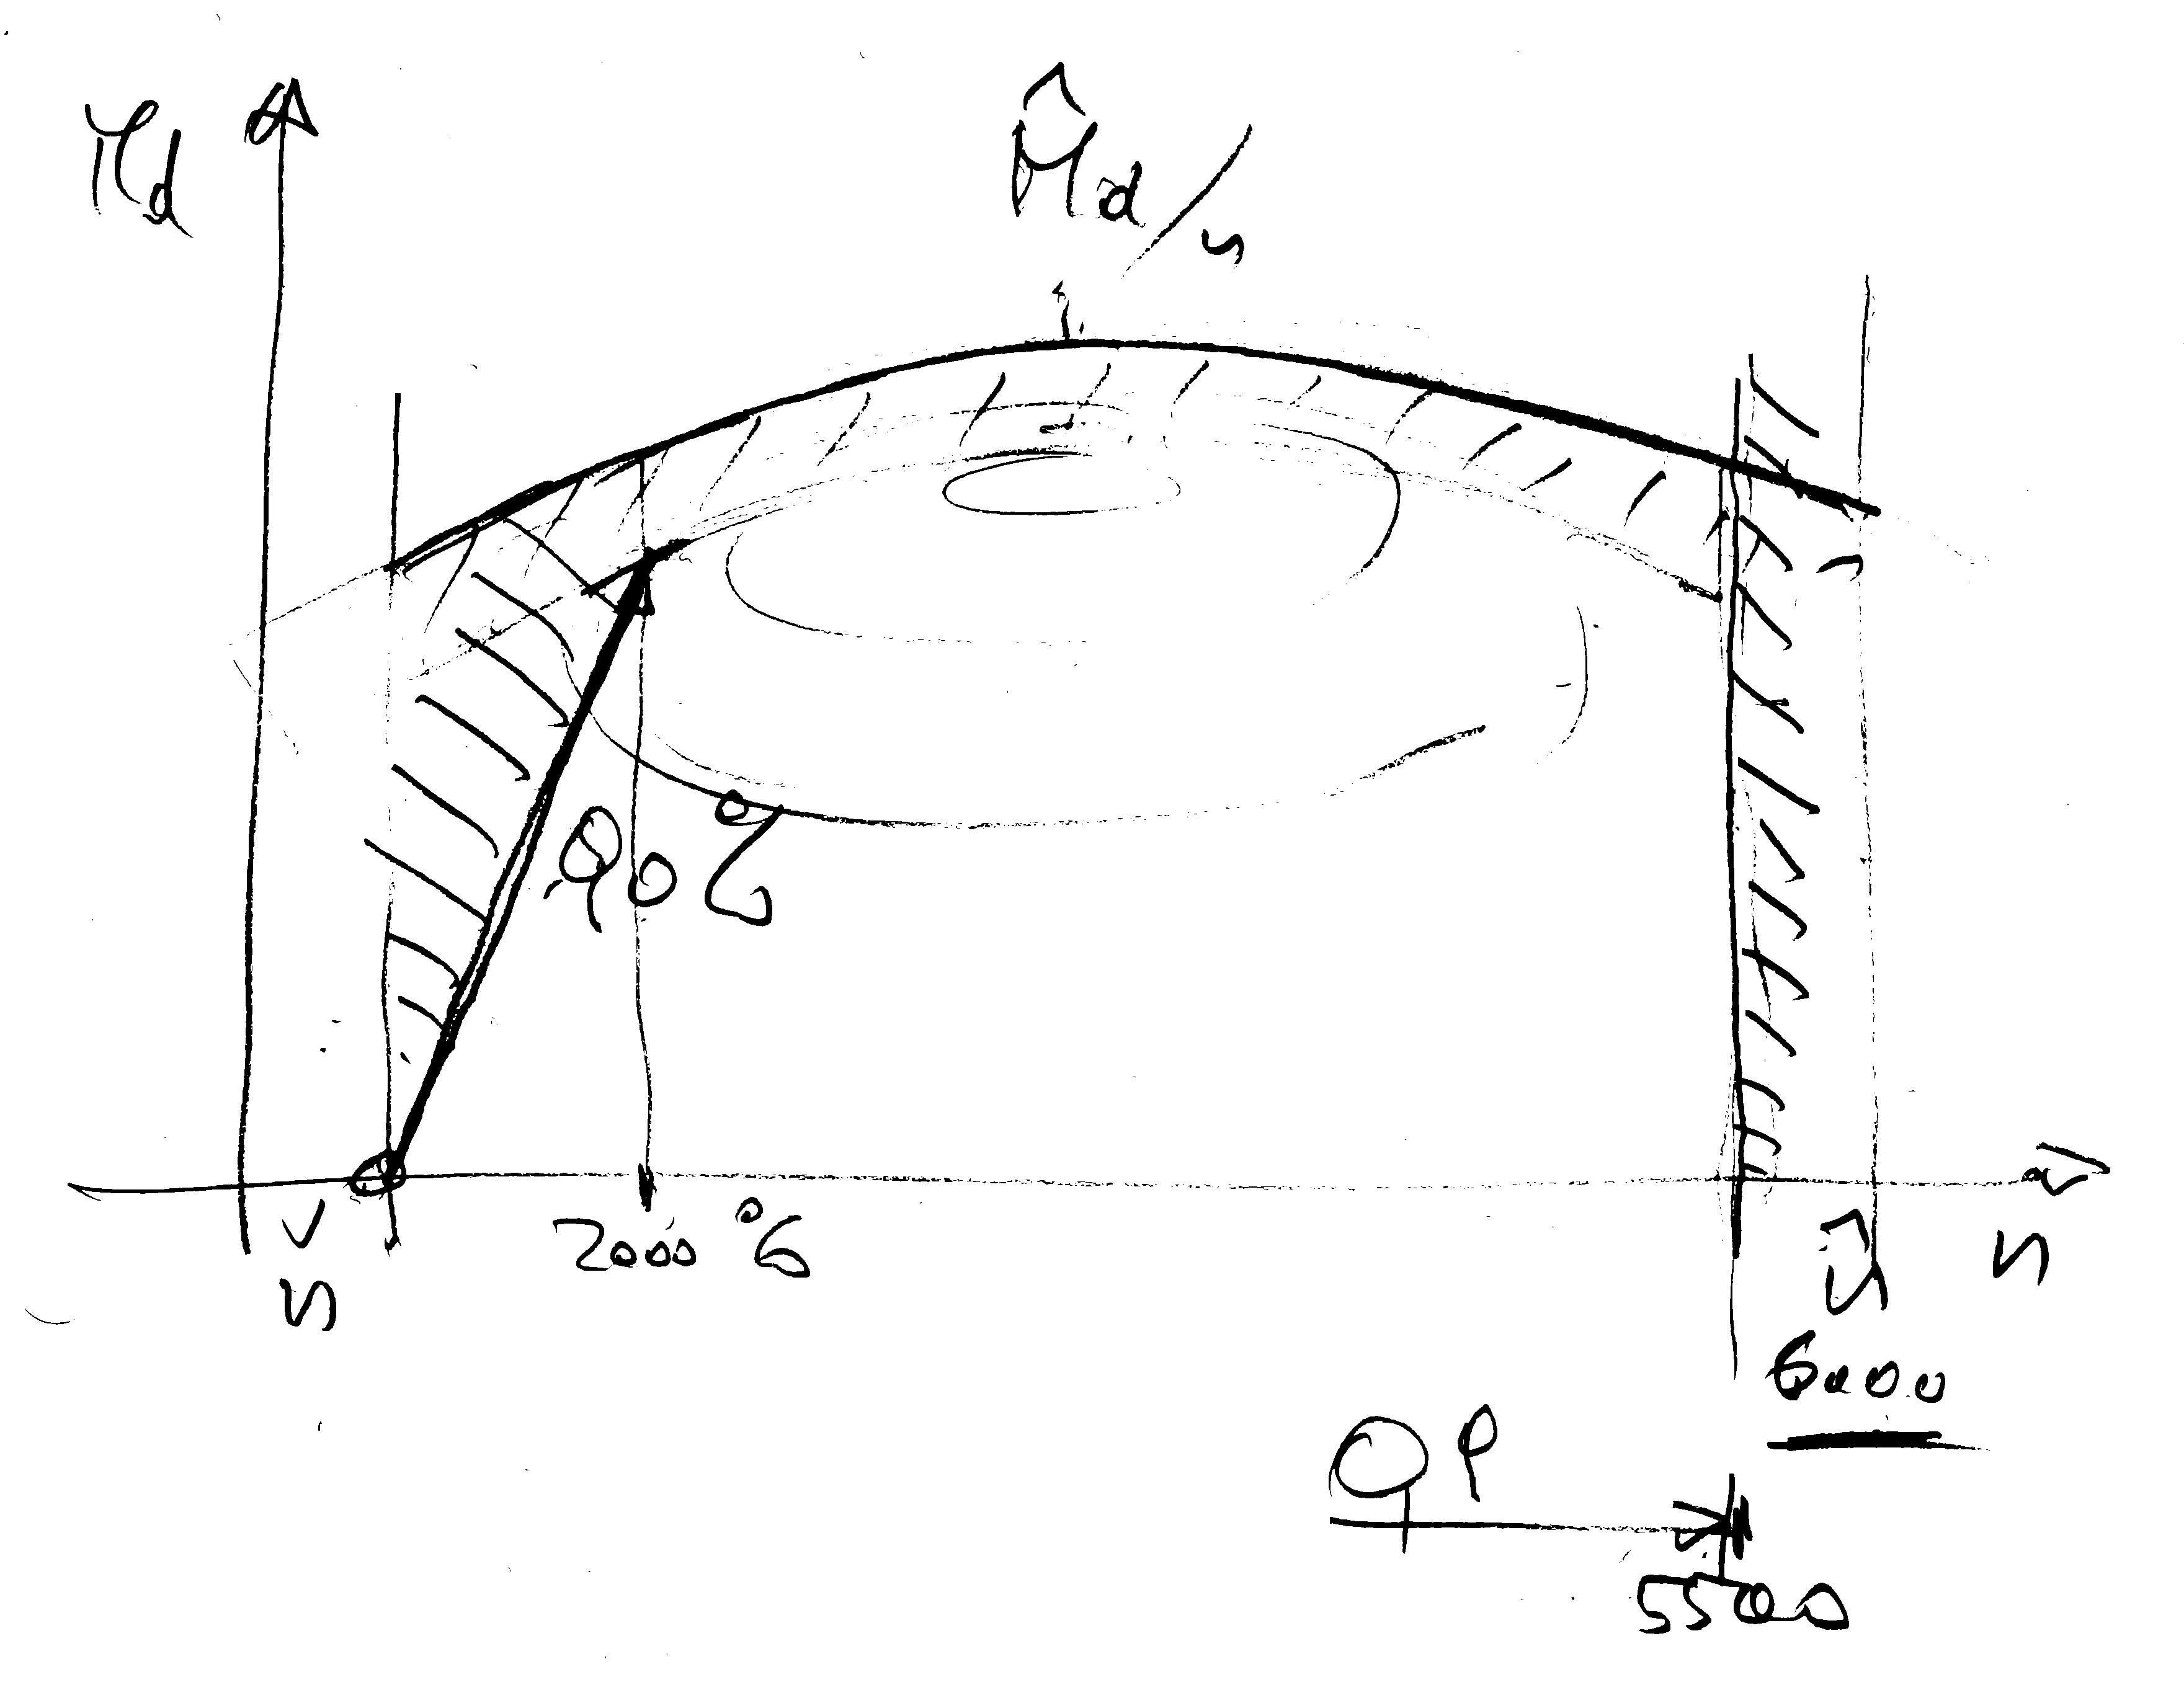
\includegraphics[width=0.8\textwidth]{images/motorkennfeldSkizze}
		\caption{Motorkennfeld mit hochschalten und hinunterschalten schattiert eingetragen} \label{fig:imgEngineEfficiencyGraph}
\end{figure}
Auf dieser Skizze erkennen Sie den Grenzwertbereich für das Hinunterschalten links, welcher aufgrund des Abriebs des Getriebes ausgelöst wird. Außerdem können Sie die Grenzwerte für das Hochschalten oben, entlang 90\% des maximalen Drehmoments auf der Drehmomentkurve und rechts entlang 90\% der maximalen Drehzahl, erkennen.

Zunächst wurde folglich überprüft, welche PID's als Basis für die weiteren Überlegungen verwendet werden könnten, um möglichst nahe an die Vorgaben aus dem Motorkennfeld zu kommen.

\lstinputlisting[caption=Output OBD-II COM-Port,firstline=1,lastline=16]{code/CH3/output.txt}
Dies ist der Output, welcher aus der OBD-II Schnittstelle erlangt wurde. Er outputted zuerst OK, dann die Nummer des PID's, das man auslesen will und darauf folgend das Ergebnis, wessen Output, wie folglich zu sehen, in einem Converter umgewandelt wird.
\begin{figure}[!htb]\centering
		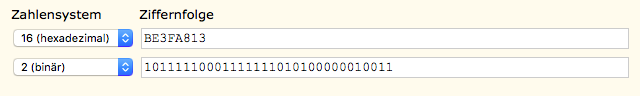
\includegraphics[width=0.8\textwidth]{images/hextoBinary}
		\caption{Umrechnung von hexadezimal zu binär\cite{SIMR.CH3-schaltvorschlag.hextoBinaryConverter}} \label{fig:imghextoBinary}
\end{figure}

Dieser binäre Code wurde, wie bereits bei 2.1.1 OBD-II, beschrieben, wird diese nun in eine Tabelle eingetragen. 
\begin{table}[!htb]
\centering
\resizebox{\columnwidth}{!}{%
\begin{tabular}{lcccccccccccccccccccccccccccccccc}
\cellcolor[HTML]{9B9B9B}Mode 01: 00-20 & \multicolumn{1}{l}{} & \multicolumn{1}{l}{} & \multicolumn{1}{l}{} & \multicolumn{1}{l}{} & \multicolumn{1}{l}{} & \multicolumn{1}{l}{} & \multicolumn{1}{l}{} & \multicolumn{1}{l}{} & \multicolumn{1}{l}{} & \multicolumn{1}{l}{} & \multicolumn{1}{l}{} & \multicolumn{1}{l}{} & \multicolumn{1}{l}{} & \multicolumn{1}{l}{} & \multicolumn{1}{l}{} & \multicolumn{1}{l}{} & \multicolumn{1}{l}{} & \multicolumn{1}{l}{} & \multicolumn{1}{l}{} & \multicolumn{1}{l}{} & \multicolumn{1}{l}{} & \multicolumn{1}{l}{} & \multicolumn{1}{l}{} & \multicolumn{1}{l}{} & \multicolumn{1}{l}{} & \multicolumn{1}{l}{} & \multicolumn{1}{l}{} & \multicolumn{1}{l}{} & \multicolumn{1}{l}{} & \multicolumn{1}{l}{} & \multicolumn{1}{l}{} & \multicolumn{1}{l}{} \\ \hline
\multicolumn{1}{|l|}{Hexadecimal} & \multicolumn{4}{c|}{B} & \multicolumn{4}{c|}{E} & \multicolumn{4}{c|}{3} & \multicolumn{4}{c|}{F} & \multicolumn{4}{c|}{A} & \multicolumn{4}{c|}{8} & \multicolumn{4}{c|}{1} & \multicolumn{4}{c|}{3} \\ \hline
\multicolumn{1}{|l|}{Binary} & \multicolumn{1}{c|}{1} & \multicolumn{1}{c|}{0} & \multicolumn{1}{c|}{1} & \multicolumn{1}{c|}{1} & \multicolumn{1}{c|}{1} & \multicolumn{1}{c|}{1} & \multicolumn{1}{c|}{1} & \multicolumn{1}{c|}{0} & \multicolumn{1}{c|}{\cellcolor[HTML]{FFFFFF}0} & \multicolumn{1}{c|}{0} & \multicolumn{1}{c|}{1} & \multicolumn{1}{c|}{1} & \multicolumn{1}{c|}{1} & \multicolumn{1}{c|}{\cellcolor[HTML]{FFFFFF}1} & \multicolumn{1}{c|}{1} & \multicolumn{1}{c|}{1} & \multicolumn{1}{c|}{\cellcolor[HTML]{9AFF99}1} & \multicolumn{1}{c|}{0} & \multicolumn{1}{c|}{1} & \multicolumn{1}{c|}{0} & \multicolumn{1}{c|}{1} & \multicolumn{1}{c|}{0} & \multicolumn{1}{c|}{0} & \multicolumn{1}{c|}{0} & \multicolumn{1}{c|}{0} & \multicolumn{1}{c|}{0} & \multicolumn{1}{c|}{0} & \multicolumn{1}{c|}{1} & \multicolumn{1}{c|}{0} & \multicolumn{1}{c|}{0} & \multicolumn{1}{c|}{1} & \multicolumn{1}{c|}{1} \\ \hline
\multicolumn{1}{|l|}{Supported?} & \multicolumn{1}{c|}{\cellcolor[HTML]{9AFF99}Yes} & \multicolumn{1}{c|}{\cellcolor[HTML]{FD6864}No} & \multicolumn{1}{c|}{\cellcolor[HTML]{9AFF99}Yes} & \multicolumn{1}{c|}{\cellcolor[HTML]{9AFF99}Yes} & \multicolumn{1}{c|}{\cellcolor[HTML]{9AFF99}Yes} & \multicolumn{1}{c|}{\cellcolor[HTML]{9AFF99}Yes} & \multicolumn{1}{c|}{\cellcolor[HTML]{9AFF99}Yes} & \multicolumn{1}{c|}{\cellcolor[HTML]{FD6864}No} & \multicolumn{1}{c|}{\cellcolor[HTML]{FD6864}No} & \multicolumn{1}{c|}{\cellcolor[HTML]{FD6864}No} & \multicolumn{1}{c|}{\cellcolor[HTML]{9AFF99}Yes} & \multicolumn{1}{c|}{\cellcolor[HTML]{9AFF99}Yes} & \multicolumn{1}{c|}{\cellcolor[HTML]{9AFF99}Yes} & \multicolumn{1}{c|}{\cellcolor[HTML]{9AFF99}Yes} & \multicolumn{1}{c|}{\cellcolor[HTML]{9AFF99}Yes} & \multicolumn{1}{c|}{\cellcolor[HTML]{9AFF99}Yes} & \multicolumn{1}{c|}{\cellcolor[HTML]{9AFF99}Yes} & \multicolumn{1}{c|}{\cellcolor[HTML]{FD6864}No} & \multicolumn{1}{c|}{\cellcolor[HTML]{9AFF99}Yes} & \multicolumn{1}{c|}{\cellcolor[HTML]{FD6864}No} & \multicolumn{1}{c|}{\cellcolor[HTML]{9AFF99}Yes} & \multicolumn{1}{c|}{\cellcolor[HTML]{FD6864}No} & \multicolumn{1}{c|}{\cellcolor[HTML]{FD6864}No} & \multicolumn{1}{c|}{\cellcolor[HTML]{FD6864}No} & \multicolumn{1}{c|}{\cellcolor[HTML]{FD6864}No} & \multicolumn{1}{c|}{\cellcolor[HTML]{FD6864}No} & \multicolumn{1}{c|}{\cellcolor[HTML]{FD6864}No} & \multicolumn{1}{c|}{\cellcolor[HTML]{9AFF99}Yes} & \multicolumn{1}{c|}{\cellcolor[HTML]{FD6864}No} & \multicolumn{1}{c|}{\cellcolor[HTML]{FD6864}No} & \multicolumn{1}{c|}{\cellcolor[HTML]{9AFF99}Yes} & \multicolumn{1}{c|}{\cellcolor[HTML]{9AFF99}Yes} \\ \hline
\multicolumn{1}{|l|}{PID number} & \multicolumn{1}{c|}{1} & \multicolumn{1}{c|}{2} & \multicolumn{1}{c|}{3} & \multicolumn{1}{c|}{4} & \multicolumn{1}{c|}{5} & \multicolumn{1}{c|}{6} & \multicolumn{1}{c|}{7} & \multicolumn{1}{c|}{8} & \multicolumn{1}{c|}{9} & \multicolumn{1}{c|}{0A} & \multicolumn{1}{c|}{0B} & \multicolumn{1}{c|}{0C} & \multicolumn{1}{c|}{0D} & \multicolumn{1}{c|}{0E} & \multicolumn{1}{c|}{0F} & \multicolumn{1}{c|}{10} & \multicolumn{1}{c|}{11} & \multicolumn{1}{c|}{12} & \multicolumn{1}{c|}{13} & \multicolumn{1}{c|}{14} & \multicolumn{1}{c|}{15} & \multicolumn{1}{c|}{16} & \multicolumn{1}{c|}{17} & \multicolumn{1}{c|}{18} & \multicolumn{1}{c|}{19} & \multicolumn{1}{c|}{1A} & \multicolumn{1}{c|}{1B} & \multicolumn{1}{c|}{1C} & \multicolumn{1}{c|}{1D} & \multicolumn{1}{c|}{1E} & \multicolumn{1}{c|}{1F} & \multicolumn{1}{c|}{20} \\ \hline
\cellcolor[HTML]{9B9B9B}Mode 01: 20-40 & \multicolumn{1}{l}{} & \multicolumn{1}{l}{} & \multicolumn{1}{l}{} & \multicolumn{1}{l}{} & \multicolumn{1}{l}{} & \multicolumn{1}{l}{} & \multicolumn{1}{l}{} & \multicolumn{1}{l}{} & \multicolumn{1}{l}{} & \multicolumn{1}{l}{} & \multicolumn{1}{l}{} & \multicolumn{1}{l}{} & \multicolumn{1}{l}{} & \multicolumn{1}{l}{\cellcolor[HTML]{FFFFFF}} & \multicolumn{1}{l}{} & \multicolumn{1}{l}{} & \multicolumn{1}{l}{} & \multicolumn{1}{l}{} & \multicolumn{1}{l}{} & \multicolumn{1}{l}{} & \multicolumn{1}{l}{} & \multicolumn{1}{l}{} & \multicolumn{1}{l}{} & \multicolumn{1}{l}{} & \multicolumn{1}{l}{} & \multicolumn{1}{l}{} & \multicolumn{1}{l}{} & \multicolumn{1}{l}{} & \multicolumn{1}{l}{} & \multicolumn{1}{l}{} & \multicolumn{1}{l}{} & \multicolumn{1}{l}{} \\ \hline
\multicolumn{1}{|l|}{Hexadecimal} & \multicolumn{4}{c|}{8} & \multicolumn{4}{c|}{0} & \multicolumn{4}{c|}{1} & \multicolumn{4}{c|}{5} & \multicolumn{4}{c|}{B} & \multicolumn{4}{c|}{0} & \multicolumn{4}{c|}{1} & \multicolumn{4}{c|}{1} \\ \hline
\multicolumn{1}{|l|}{Binary} & \multicolumn{1}{c|}{1} & \multicolumn{1}{c|}{0} & \multicolumn{1}{c|}{0} & \multicolumn{1}{c|}{0} & \multicolumn{1}{c|}{0} & \multicolumn{1}{c|}{0} & \multicolumn{1}{c|}{0} & \multicolumn{1}{c|}{0} & \multicolumn{1}{c|}{0} & \multicolumn{1}{c|}{0} & \multicolumn{1}{c|}{0} & \multicolumn{1}{c|}{1} & \multicolumn{1}{c|}{0} & \multicolumn{1}{c|}{1} & \multicolumn{1}{c|}{0} & \multicolumn{1}{c|}{1} & \multicolumn{1}{c|}{1} & \multicolumn{1}{c|}{0} & \multicolumn{1}{c|}{1} & \multicolumn{1}{c|}{1} & \multicolumn{1}{c|}{0} & \multicolumn{1}{c|}{0} & \multicolumn{1}{c|}{0} & \multicolumn{1}{c|}{0} & \multicolumn{1}{c|}{0} & \multicolumn{1}{c|}{0} & \multicolumn{1}{c|}{0} & \multicolumn{1}{c|}{1} & \multicolumn{1}{c|}{0} & \multicolumn{1}{c|}{0} & \multicolumn{1}{c|}{0} & \multicolumn{1}{c|}{1} \\ \hline
\multicolumn{1}{|l|}{Supported?} & \multicolumn{1}{c|}{\cellcolor[HTML]{9AFF99}Yes} & \multicolumn{1}{c|}{\cellcolor[HTML]{FD6864}No} & \multicolumn{1}{c|}{\cellcolor[HTML]{FD6864}No} & \multicolumn{1}{c|}{\cellcolor[HTML]{FD6864}No} & \multicolumn{1}{c|}{\cellcolor[HTML]{FD6864}No} & \multicolumn{1}{c|}{\cellcolor[HTML]{FD6864}No} & \multicolumn{1}{c|}{\cellcolor[HTML]{FD6864}No} & \multicolumn{1}{c|}{\cellcolor[HTML]{FD6864}No} & \multicolumn{1}{c|}{\cellcolor[HTML]{FD6864}No} & \multicolumn{1}{c|}{\cellcolor[HTML]{FD6864}No} & \multicolumn{1}{c|}{\cellcolor[HTML]{FD6864}No} & \multicolumn{1}{c|}{\cellcolor[HTML]{9AFF99}Yes} & \multicolumn{1}{c|}{\cellcolor[HTML]{FD6864}No} & \multicolumn{1}{c|}{\cellcolor[HTML]{9AFF99}Yes} & \multicolumn{1}{c|}{\cellcolor[HTML]{FD6864}No} & \multicolumn{1}{c|}{\cellcolor[HTML]{9AFF99}Yes} & \multicolumn{1}{c|}{\cellcolor[HTML]{9AFF99}Yes} & \multicolumn{1}{c|}{\cellcolor[HTML]{FD6864}No} & \multicolumn{1}{c|}{\cellcolor[HTML]{9AFF99}Yes} & \multicolumn{1}{c|}{\cellcolor[HTML]{9AFF99}Yes} & \multicolumn{1}{c|}{\cellcolor[HTML]{FD6864}No} & \multicolumn{1}{c|}{\cellcolor[HTML]{FD6864}No} & \multicolumn{1}{c|}{\cellcolor[HTML]{FD6864}No} & \multicolumn{1}{c|}{\cellcolor[HTML]{FD6864}No} & \multicolumn{1}{c|}{\cellcolor[HTML]{FD6864}No} & \multicolumn{1}{c|}{\cellcolor[HTML]{FD6864}No} & \multicolumn{1}{c|}{\cellcolor[HTML]{FD6864}No} & \multicolumn{1}{c|}{\cellcolor[HTML]{9AFF99}Yes} & \multicolumn{1}{c|}{\cellcolor[HTML]{FD6864}No} & \multicolumn{1}{c|}{\cellcolor[HTML]{FD6864}No} & \multicolumn{1}{c|}{\cellcolor[HTML]{FD6864}No} & \multicolumn{1}{c|}{\cellcolor[HTML]{9AFF99}Yes} \\ \hline
\multicolumn{1}{|l|}{PID number} & \multicolumn{1}{c|}{21} & \multicolumn{1}{c|}{22} & \multicolumn{1}{c|}{23} & \multicolumn{1}{c|}{24} & \multicolumn{1}{c|}{25} & \multicolumn{1}{c|}{26} & \multicolumn{1}{c|}{27} & \multicolumn{1}{c|}{28} & \multicolumn{1}{c|}{29} & \multicolumn{1}{c|}{2a} & \multicolumn{1}{c|}{2b} & \multicolumn{1}{c|}{2c} & \multicolumn{1}{c|}{2d} & \multicolumn{1}{c|}{2e} & \multicolumn{1}{c|}{2f} & \multicolumn{1}{c|}{30} & \multicolumn{1}{c|}{31} & \multicolumn{1}{c|}{32} & \multicolumn{1}{c|}{33} & \multicolumn{1}{c|}{34} & \multicolumn{1}{c|}{35} & \multicolumn{1}{c|}{36} & \multicolumn{1}{c|}{37} & \multicolumn{1}{c|}{38} & \multicolumn{1}{c|}{39} & \multicolumn{1}{c|}{3a} & \multicolumn{1}{c|}{3b} & \multicolumn{1}{c|}{3c} & \multicolumn{1}{c|}{3d} & \multicolumn{1}{c|}{3e} & \multicolumn{1}{c|}{3f} & \multicolumn{1}{c|}{40} \\ \hline
\cellcolor[HTML]{9B9B9B}Mode 01: 40-60 & \multicolumn{1}{l}{} & \multicolumn{1}{l}{} & \multicolumn{1}{l}{} & \multicolumn{1}{l}{} & \multicolumn{1}{l}{} & \multicolumn{1}{l}{} & \multicolumn{1}{l}{} & \multicolumn{1}{l}{} & \multicolumn{1}{l}{} & \multicolumn{1}{l}{} & \multicolumn{1}{l}{} & \multicolumn{1}{l}{} & \multicolumn{1}{l}{} & \multicolumn{1}{l}{} & \multicolumn{1}{l}{} & \multicolumn{1}{l}{} & \multicolumn{1}{l}{} & \multicolumn{1}{l}{} & \multicolumn{1}{l}{} & \multicolumn{1}{l}{} & \multicolumn{1}{l}{} & \multicolumn{1}{l}{} & \multicolumn{1}{l}{} & \multicolumn{1}{l}{} & \multicolumn{1}{l}{} & \multicolumn{1}{l}{} & \multicolumn{1}{l}{} & \multicolumn{1}{l}{} & \multicolumn{1}{l}{} & \multicolumn{1}{l}{} & \multicolumn{1}{l}{} & \multicolumn{1}{l}{} \\ \hline
\multicolumn{1}{|l|}{Hexadecimal} & \multicolumn{4}{c|}{F} & \multicolumn{4}{c|}{A} & \multicolumn{4}{c|}{D} & \multicolumn{4}{c|}{0} & \multicolumn{4}{c|}{0} & \multicolumn{4}{c|}{0} & \multicolumn{4}{c|}{0} & \multicolumn{4}{c|}{0} \\ \hline
\multicolumn{1}{|l|}{Binary} & \multicolumn{1}{c|}{1} & \multicolumn{1}{c|}{1} & \multicolumn{1}{c|}{1} & \multicolumn{1}{c|}{1} & \multicolumn{1}{c|}{1} & \multicolumn{1}{c|}{0} & \multicolumn{1}{c|}{1} & \multicolumn{1}{c|}{0} & \multicolumn{1}{c|}{1} & \multicolumn{1}{c|}{1} & \multicolumn{1}{c|}{0} & \multicolumn{1}{c|}{1} & \multicolumn{1}{c|}{0} & \multicolumn{1}{c|}{0} & \multicolumn{1}{c|}{0} & \multicolumn{1}{c|}{0} & \multicolumn{1}{c|}{0} & \multicolumn{1}{c|}{0} & \multicolumn{1}{c|}{0} & \multicolumn{1}{c|}{0} & \multicolumn{1}{c|}{0} & \multicolumn{1}{c|}{0} & \multicolumn{1}{c|}{0} & \multicolumn{1}{c|}{0} & \multicolumn{1}{c|}{0} & \multicolumn{1}{c|}{0} & \multicolumn{1}{c|}{0} & \multicolumn{1}{c|}{0} & \multicolumn{1}{c|}{0} & \multicolumn{1}{c|}{0} & \multicolumn{1}{c|}{0} & \multicolumn{1}{c|}{0} \\ \hline
\multicolumn{1}{|l|}{Supported?} & \multicolumn{1}{c|}{\cellcolor[HTML]{9AFF99}Yes} & \multicolumn{1}{c|}{\cellcolor[HTML]{9AFF99}Yes} & \multicolumn{1}{c|}{\cellcolor[HTML]{9AFF99}Yes} & \multicolumn{1}{c|}{\cellcolor[HTML]{9AFF99}Yes} & \multicolumn{1}{c|}{\cellcolor[HTML]{9AFF99}Yes} & \multicolumn{1}{c|}{\cellcolor[HTML]{FD6864}No} & \multicolumn{1}{c|}{\cellcolor[HTML]{9AFF99}Yes} & \multicolumn{1}{c|}{\cellcolor[HTML]{FD6864}No} & \multicolumn{1}{c|}{\cellcolor[HTML]{9AFF99}Yes} & \multicolumn{1}{c|}{\cellcolor[HTML]{9AFF99}Yes} & \multicolumn{1}{c|}{\cellcolor[HTML]{FD6864}No} & \multicolumn{1}{c|}{\cellcolor[HTML]{9AFF99}Yes} & \multicolumn{1}{c|}{\cellcolor[HTML]{FD6864}No} & \multicolumn{1}{c|}{\cellcolor[HTML]{FD6864}No} & \multicolumn{1}{c|}{\cellcolor[HTML]{FD6864}No} & \multicolumn{1}{c|}{\cellcolor[HTML]{FD6864}No} & \multicolumn{1}{c|}{\cellcolor[HTML]{FD6864}No} & \multicolumn{1}{c|}{\cellcolor[HTML]{FD6864}No} & \multicolumn{1}{c|}{\cellcolor[HTML]{FD6864}No} & \multicolumn{1}{c|}{\cellcolor[HTML]{FD6864}No} & \multicolumn{1}{c|}{\cellcolor[HTML]{FD6864}No} & \multicolumn{1}{c|}{\cellcolor[HTML]{FD6864}No} & \multicolumn{1}{c|}{\cellcolor[HTML]{FD6864}No} & \multicolumn{1}{c|}{\cellcolor[HTML]{FD6864}No} & \multicolumn{1}{c|}{\cellcolor[HTML]{FD6864}No} & \multicolumn{1}{c|}{\cellcolor[HTML]{FD6864}No} & \multicolumn{1}{c|}{\cellcolor[HTML]{FD6864}No} & \multicolumn{1}{c|}{\cellcolor[HTML]{FD6864}No} & \multicolumn{1}{c|}{\cellcolor[HTML]{FD6864}No} & \multicolumn{1}{c|}{\cellcolor[HTML]{FD6864}No} & \multicolumn{1}{c|}{\cellcolor[HTML]{FD6864}No} & \multicolumn{1}{c|}{\cellcolor[HTML]{FD6864}No} \\ \hline
\multicolumn{1}{|l|}{PID number} & \multicolumn{1}{c|}{41} & \multicolumn{1}{c|}{42} & \multicolumn{1}{c|}{43} & \multicolumn{1}{c|}{44} & \multicolumn{1}{c|}{45} & \multicolumn{1}{c|}{46} & \multicolumn{1}{c|}{47} & \multicolumn{1}{c|}{48} & \multicolumn{1}{c|}{49} & \multicolumn{1}{c|}{4a} & \multicolumn{1}{c|}{4b} & \multicolumn{1}{c|}{4c} & \multicolumn{1}{c|}{4d} & \multicolumn{1}{c|}{4e} & \multicolumn{1}{c|}{4f} & \multicolumn{1}{c|}{50} & \multicolumn{1}{c|}{51} & \multicolumn{1}{c|}{52} & \multicolumn{1}{c|}{53} & \multicolumn{1}{c|}{54} & \multicolumn{1}{c|}{55} & \multicolumn{1}{c|}{56} & \multicolumn{1}{c|}{57} & \multicolumn{1}{c|}{58} & \multicolumn{1}{c|}{59} & \multicolumn{1}{c|}{5a} & \multicolumn{1}{c|}{5b} & \multicolumn{1}{c|}{5c} & \multicolumn{1}{c|}{5d} & \multicolumn{1}{c|}{5e} & \multicolumn{1}{c|}{5f} & \multicolumn{1}{c|}{60} \\ \hline
\cellcolor[HTML]{9B9B9B}Mode 01: 60-100 & \multicolumn{1}{l}{} & \multicolumn{1}{l}{} & \multicolumn{1}{l}{} & \multicolumn{1}{l}{} & \multicolumn{1}{l}{} & \multicolumn{1}{l}{} & \multicolumn{1}{l}{} & \multicolumn{1}{l}{} & \multicolumn{1}{l}{} & \multicolumn{1}{l}{} & \multicolumn{1}{l}{} & \multicolumn{1}{l}{} & \multicolumn{1}{l}{} & \multicolumn{1}{l}{} & \multicolumn{1}{l}{} & \multicolumn{1}{l}{} & \multicolumn{1}{l}{} & \multicolumn{1}{l}{} & \multicolumn{1}{l}{} & \multicolumn{1}{l}{} & \multicolumn{1}{l}{} & \multicolumn{1}{l}{} & \multicolumn{1}{l}{} & \multicolumn{1}{l}{} & \multicolumn{1}{l}{} & \multicolumn{1}{l}{} & \multicolumn{1}{l}{} & \multicolumn{1}{l}{} & \multicolumn{1}{l}{} & \multicolumn{1}{l}{} & \multicolumn{1}{l}{} & \multicolumn{1}{l}{} \\ \cline{1-1}
\multicolumn{1}{|l|}{NO DATA} & \multicolumn{1}{l}{} & \multicolumn{1}{l}{} & \multicolumn{1}{l}{} & \multicolumn{1}{l}{} & \multicolumn{1}{l}{} & \multicolumn{1}{l}{} & \multicolumn{1}{l}{} & \multicolumn{1}{l}{} & \multicolumn{1}{l}{} & \multicolumn{1}{l}{} & \multicolumn{1}{l}{} & \multicolumn{1}{l}{} & \multicolumn{1}{l}{} & \multicolumn{1}{l}{} & \multicolumn{1}{l}{} & \multicolumn{1}{l}{} & \multicolumn{1}{l}{} & \multicolumn{1}{l}{} & \multicolumn{1}{l}{} & \multicolumn{1}{l}{} & \multicolumn{1}{l}{} & \multicolumn{1}{l}{} & \multicolumn{1}{l}{} & \multicolumn{1}{l}{} & \multicolumn{1}{l}{} & \multicolumn{1}{l}{} & \multicolumn{1}{l}{} & \multicolumn{1}{l}{} & \multicolumn{1}{l}{} & \multicolumn{1}{l}{} & \multicolumn{1}{l}{} & \multicolumn{1}{l}{} \\ \cline{1-1}
\end{tabular}}
\caption{Tabelle der verfügbaren PID's unseres Mazda3}
\label{tableMazda3}
\end{table}

Durch die Tabelle war es uns erstmals möglich zu erkennen, welche Daten wir auslesen können. Bei genauerer Betrachtung der OBD-II PID's schlussfolgerten wir, dass es keine Möglichkeit geben wird den Gang auszulesen, ohne dabei unverhältnismäßige Aufwände aufzuwenden. Diese Aufwände wären von komplexen mathematischen Schlussfolgerungen, bis hin zur Modifikation unseres Testfahrzeugs gegangen. Stattdessen einigte sich das Team darauf, sich nur mit einem Vorschlag nach oben oder unten zufrieden zu geben. 

Zum Zweck des Gangvorschlags werden 2 PID's benötigt. Diese findet man perfekt in Wikipedia's OBD-II PID'-spage aufgeschlüsselt wieder, wofür das Geld weiter verwendet wird.
\begin{itemize}
	\item Mode 01 PID 04: calculated engine load [0-100[\%]], auf der vertikalen Achse
	\item Mode 01 PID 0C: engine rpm [[0-16,383.75]rpm], auf der horizontalen Achse
\end{itemize} 

Durch diese Variablen muss eine Klassenbildung für das herunterschalten umgesetzt werden, da es hier kein einzelnes Maß gibt auf welches man ein überschreiten des Maximums schließen könnte. Beim heraufschalten Wiederrum, wird keine Klassenbildung benötigt da hier entweder zuerst 90\% des möglichen Drehmoments oder der nötigen Drehzahl getroffen werden. Ausserdem ist die calculated engine load eine Prozentzahl. 

\subsubsection{Designüberlegung}
Zuerst wurde überlegt wie man einen Schaltvorschlag designen kann. 
Bei der Designüberlegung kam vor allem zu tragen, dass das Design so einfach zu bedienen sein sollte, dass es den Fahrer möglichst gar nicht ablenkt. Weiters muss durch die fehlende Unterstützung für Schaltgetriebe, händisch in einer Settingpane eingegeben werden wie hoch die maximale Drehzahl des Motors ist. (Diesel und Benzin stark unterschiedliche maximale Drehazahlen!) Zusätzlich dazu wurde überlegt, wie man am intuitivsten hinauf oder hinunterschalten anzeigt.

Für das Design wurde überlegt ob ein Drehzahlmesser auf der Android Applikation klug wäre, wofür sich letztendlich doch entschieden wurde. Denn man bekommt mit diesem auch selbst ein Gefühl für das Schalten bekommen kann und sich mit der Zeit merken wird, wann man in welchen Gang schalten sollte. Ausserdem wird ein Pfeil eingesetzt, welcher die Richtung wechselt oder komplett auf ein X wechselt, so keine Aktion ergriffen werden soll. Dies haben alle Probanden ohne weiterer Erklärung als dem Kontext unserer App auf Anhieb verstanden. Es wurden folglich also Gauge Libraries evaluiert, um möglichst die perfekte Library zu benutzen.

\subsubsection{Umsetzung}
Der Stand der Technik ist nur bezüglich unserer eigenen Hardware äußerst modern, viele der ECU's sind 10 Jahre oder älter. Daher ist auch das Auslesen der Schnittstelle sehr einfach zu handhaben. Als direkte Konkurrenz war kein Produkt auffindbar.
Im Bezug auf meinen Lösungsweg des Schaltvorschlags war ich sehr eingeschränkt, da ich nur den Lösungsweg, welchen mir Prof. Neuburger näher gebracht hat, einsetzen konnte. Bezüglich der Android App hatte ich andererseits vollkommene gestalterische Freiheit, hier wurden die Ansätze gewählt, welche am besten dokumentiert sind.
Um diese beiden Teile zu realisieren, wurden mehrere Libraries verwendet, die alle ausschließlich Android Studio verwenden.
Einerseits wurde GaugeView for Lollipop \cite{SIMR.CH3-schaltvorschlag.GaugeView} verwendet, andererseits wurde mittels ImageCircleView \cite{SIMR.CH3-schaltvorschlag.CircleImageView} das Bild des Pfeils und des Kreuzes dargestellt.
Ausserdem musste eine SettingsPane umgesetzt werden, in welcher man die maximale Drehzahl verstellen kann, implementiert werden.
Es wurde die App mittels Gradle und der Android SDK 23 umgesetzt.

Probleme kamen vor allem beim Aufbau der GaugeView Library auf, welche ich aufgrund eines doppelten XML attributes (showText) händisch zu einem Android Library Package (.aar) kompilieren musste, damit ich diesen Fehler umgehen konnte, eine schönere Lösung hierfür wurde bisweilen noch nicht vom Library-Ersteller bereitet. 
\begin{figure}[!htb]\centering
		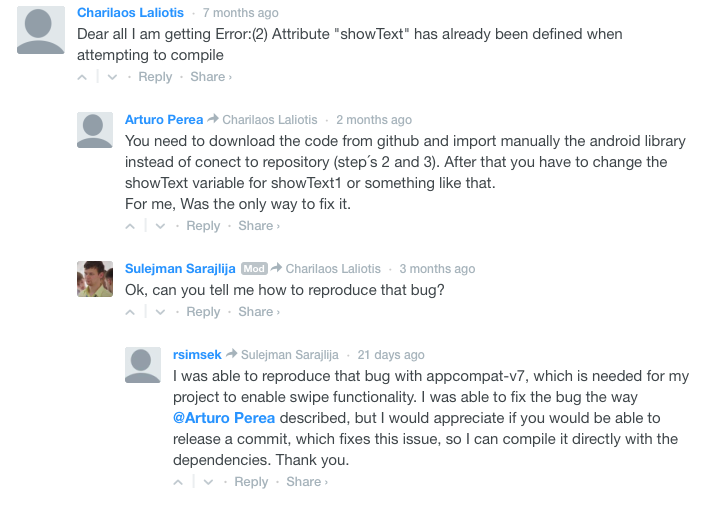
\includegraphics[width=0.75\textwidth]{images/gaugeViewShowText}
		\caption{Disqus Chat zu showText bei GaugeView} \label{fig:imgGaugeViewDisqus}
\end{figure}

\lstinputlisting[caption=shift XML design file,firstline=1,lastline=40,style=xmlstyle]{code/CH3/schalt.xml}

\begin{figure}[!htb]\centering
		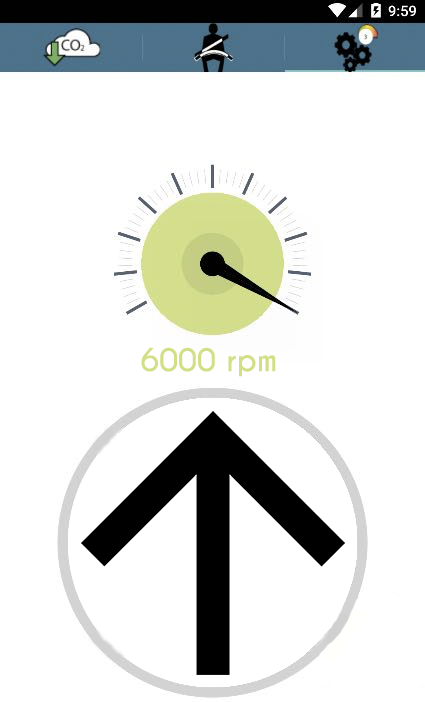
\includegraphics[width=0.3\textwidth]{images/schalt}
		\caption{finale Umsetzung der Android App beim Schaltvorschlag} \label{fig:imgShiftAndroidFinished}
\end{figure}


\clearpage % DO NOT REMOVE